% Standalone insertion fragment; add \usepackage{graphicx} to the preamble.
% Keep xe133_xe131m_ellipse.pdf beside the manuscript, or adjust its path.
\begin{figure*}[t]
  \centering
  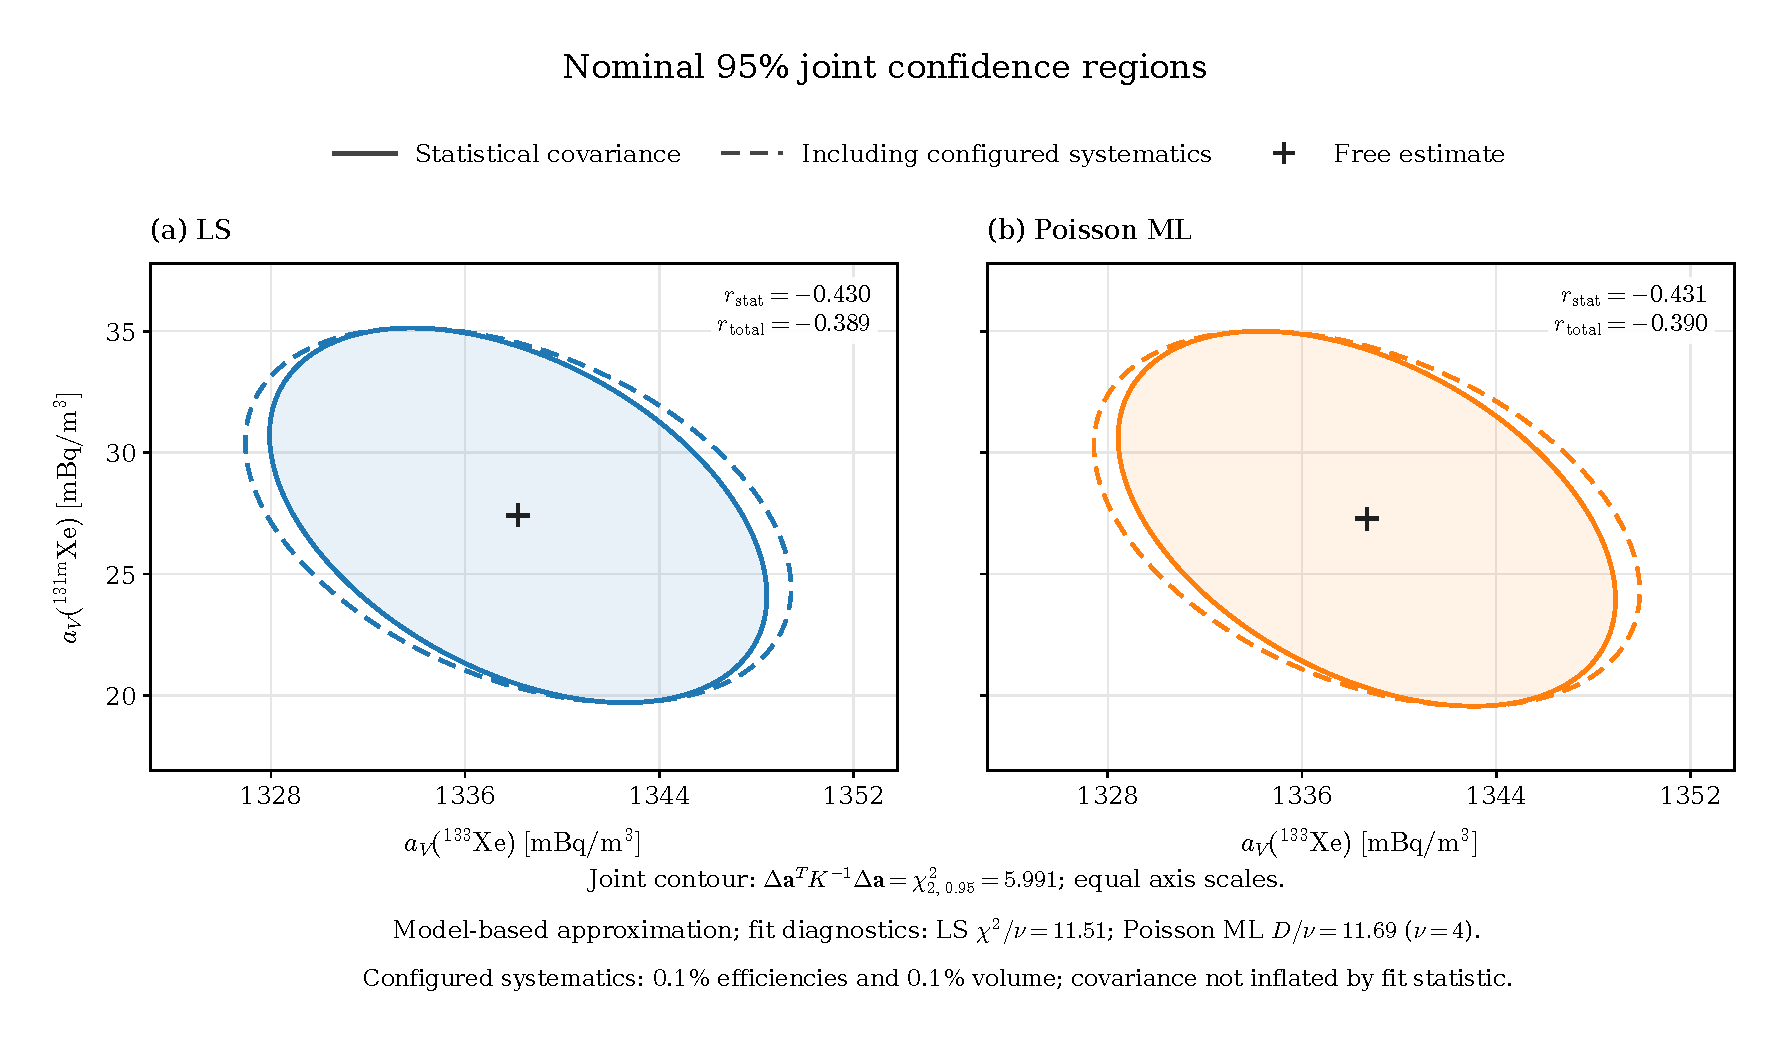
\includegraphics[width=\textwidth]{xe133_xe131m_ellipse.pdf}
  \caption{Nominal joint 95\% confidence regions for the fresh-sample
  concentrations of $^{133}$Xe and $^{131\mathrm{m}}$Xe, obtained by
  (a) weighted least squares and (b) unconstrained Poisson maximum likelihood.
  Both methods use the original detector-221 responses, fixed efficiencies
  and ROI, and the joint SAMPLE/GASBK/DETBK model for the August measurement.
  The two-coordinate covariance block is extracted after accounting for all
  fitted nuisance parameters, including gas memory and detector background.
  Solid contours use statistical covariance; dashed contours additionally
  include the configured propagated uncertainties of 0.1\% in efficiencies
  and 0.1\% in volume. Crosses mark the free estimates; the negative
  correlation tilts the regions downward. Each contour satisfies
  $\Delta\mathbf{a}^{T}K^{-1}\Delta\mathbf{a}=\chi^2_{2,0.95}=5.991$.
  Axes have equal scales and are enlarged around the estimates.
  These are normal-approximation, model-based regions: the reduced
  fit statistics are 11.51 and 11.69, respectively, so the nominal 95\%
  coverage is not established for these real spectra. The covariances
  have not been rescaled by the fit statistics.}
  \label{fig:xemat-august-xe133-xe131m}
\end{figure*}
